\chapter{[matplotlib] 图片样式与排版}
\section{默认配置}
matplotlib 的相关配置主要包括以下几种，用户可以自定义它们：
\begin{enumerate}[label=\arabic*)]
    \item 图片大小(\codeinline{figsize})和分辨率(\codeinline{dpi})
    \item 线宽(\codeinline{linewidth})、颜色(\codeinline{color})、风格(\codeinline{linestyle})和标记(\codeinline{marker})
    \item 坐标轴(\codeinline{axis})、坐标轴标签(\codeinline{xlabel, ylabel})以及网格(\codeinline{grid})的属性
    \item 文字(\codeinline{text})与字体(\codeinline{font})属性。
\end{enumerate}

所有的默认属性均保存在 \codeinline{matplotlib.rcParams} 字典中。
\begin{lstlisting}[style=pythonstyle]
import matplotlib.pyplot as plt

# 查看所有的 rcParams 及其默认值
for key, value in plt.rcParams.items():
    print(f"{key}: {value}")
\end{lstlisting}    

可以对 \codeinline{plt.rcParams} 进行修改，以\textcolor{red}{\textbf{全局}}改变默认的配置。例如，修改图片的尺寸和分辨率：
\begin{lstlisting}[style=pythonstyle]
import matplotlib.pyplot as plt

# 查看特定的 rcParams 值
print(plt.rcParams['figure.figsize'])  # 图像尺寸
print(plt.rcParams['figure.dpi'])      # 图像分辨率
print(plt.rcParams['lines.linewidth']) # 线条宽度

# 修改默认的图像尺寸和分辨率
plt.rcParams['figure.figsize'] = [10, 6]
plt.rcParams['figure.dpi'] = 120
print(plt.rcParams['figure.figsize'])  # 图像尺寸
print(plt.rcParams['figure.dpi'])      # 图像分辨率

# 绘制一个简单的图形，使用新的设置
plt.plot([1, 2, 3, 4], [1, 4, 2, 3])
plt.show()
\end{lstlisting}   

如果不想全局修改默认配置，可以使用 \codeinline{plt.rc()} 函数来临时修改配置：
\begin{lstlisting}[style=pythonstyle]
import matplotlib.pyplot as plt  
plt.figure(figsize=(10, 6), dpi=120)  
plt.plot([1, 2, 3, 4], [1, 4, 2, 3])
plt.show()
\end{lstlisting}

\section{显示中文}
\begin{lstlisting}[style=demostyle,numbers=none]
# 1.定位matplotlib的字体库路径
import matplotlib
matplotlib.matplotlib_fname()
>>> '/home/changjie/.local/conda_env/pytorch_test/lib/python3.10/site-packages/matplotlib/mpl-data/matplotlibrc'

# 2.将中文字体文件**.ttf，拷贝到该目录的fonts/ttf下
cp /usr/share/fonts/emacs_cnfonts/chinese/* /home/changjie/.local/conda_env/pytorch_test/lib/python3.10/site-packages/matplotlib/mpl-data/fonts/ttf/

# 3删除 matplotlib 缓存
cd ~/.cache/matplotlib
rm * -r

# 4.查看是否成功
import matplotlib.pyplot as plt  
from matplotlib import font_manager  
# 获取字体管理器并列出所有TTF字体  
fonts = [f.name for f in font_manager.fontManager.ttflist]  
sorted_fonts = sorted(fonts)  
# 打印排序后的字体列表  
print(sorted_fonts)

# 5.使用字体
## 1)用plt.rcParams设置
plt.rcParams['font.family'] = 'SimSun'   
plt.rcParams['axes.unicode_minus'] = False  # 解决保存图像时负号'-'显示为方块的问题

## 2)用FontProperties，并指定字体文件
from matplotlib.font_manager import FontProperties
import matplotlib.pyplot as plt
font = FontProperties(fname='/mnt/share/code/font/SimHei.ttf', size=20)
plt.title('测试', fontproperties=font)
\end{lstlisting}  

\section{图片的属性}
\begin{table}[h]
    \centering
    \begin{tabular}{|c|c|l|}
    \hline
    \textbf{参数} & \textbf{默认值} & \textbf{描述}                 \\ \hline
    num           & 1               & 图像的数量                   \\ \hline
    figsize       & figure.figsize  & 图像的长和宽（英寸）         \\ \hline
    dpi           & figure.dpi      & 分辨率（像素/英寸）           \\ \hline
    facecolor     & figure.facecolor & 绘图区域的背景颜色           \\ \hline
    edgecolor     & figure.edgecolor & 绘图区域边缘的颜色           \\ \hline
    frameon       & True            & 是否绘制图像边缘             \\ \hline
    \end{tabular}
    \caption{图像的属性}
\end{table}

高 dpi 显示图像更细腻，但是图像尺寸也会变大。使用默认值即可。如果图像非常复杂，为了看清细节，我们可以调整宽高的英寸数。

\begin{lstlisting}[style=pythonstyle]
import matplotlib.pyplot as plt
plt.rcParams['font.family'] = 'SimSun'   

# 示例 1：默认参数
plt.figure(num=1)
plt.plot([0, 1, 2], [0, 1, 4], label='默认参数')
plt.title('默认参数')
plt.legend()
plt.show()

# 示例 2：设置图像大小（figsize）
plt.figure(num=2, figsize=(10, 5))
plt.plot([0, 1, 2], [0, 1, 4], label='figsize = (10, 5)')
plt.title('设置图像大小')
plt.legend()
plt.show()

# 示例 3：设置分辨率（dpi）
plt.figure(num=3, dpi=150)
plt.plot([0, 1, 2], [0, 1, 4], label='dpi = 150')
plt.title('设置分辨率')
plt.legend()
plt.show()

# 示例 4：设置背景颜色（facecolor）
plt.figure(num=4, facecolor='lightgray')
plt.plot([0, 1, 2], [0, 1, 4], label='facecolor = lightgray')
plt.title('设置背景颜色')
plt.legend()
plt.show()

# 示例 5：设置边缘颜色（edgecolor）
plt.figure(num=5, edgecolor='red')
plt.plot([0, 1, 2], [0, 1, 4], label='edgecolor = red')
plt.title('设置边缘颜色')
plt.legend()
plt.show()

# 示例 6：关闭边框（frameon=False）
plt.figure(num=6, frameon=False)
plt.plot([0, 1, 2], [0, 1, 4], label='frameon = False')
plt.title('关闭边框')
plt.legend()
plt.show()
\end{lstlisting}

\begin{figure}[htpb]
    \centering
    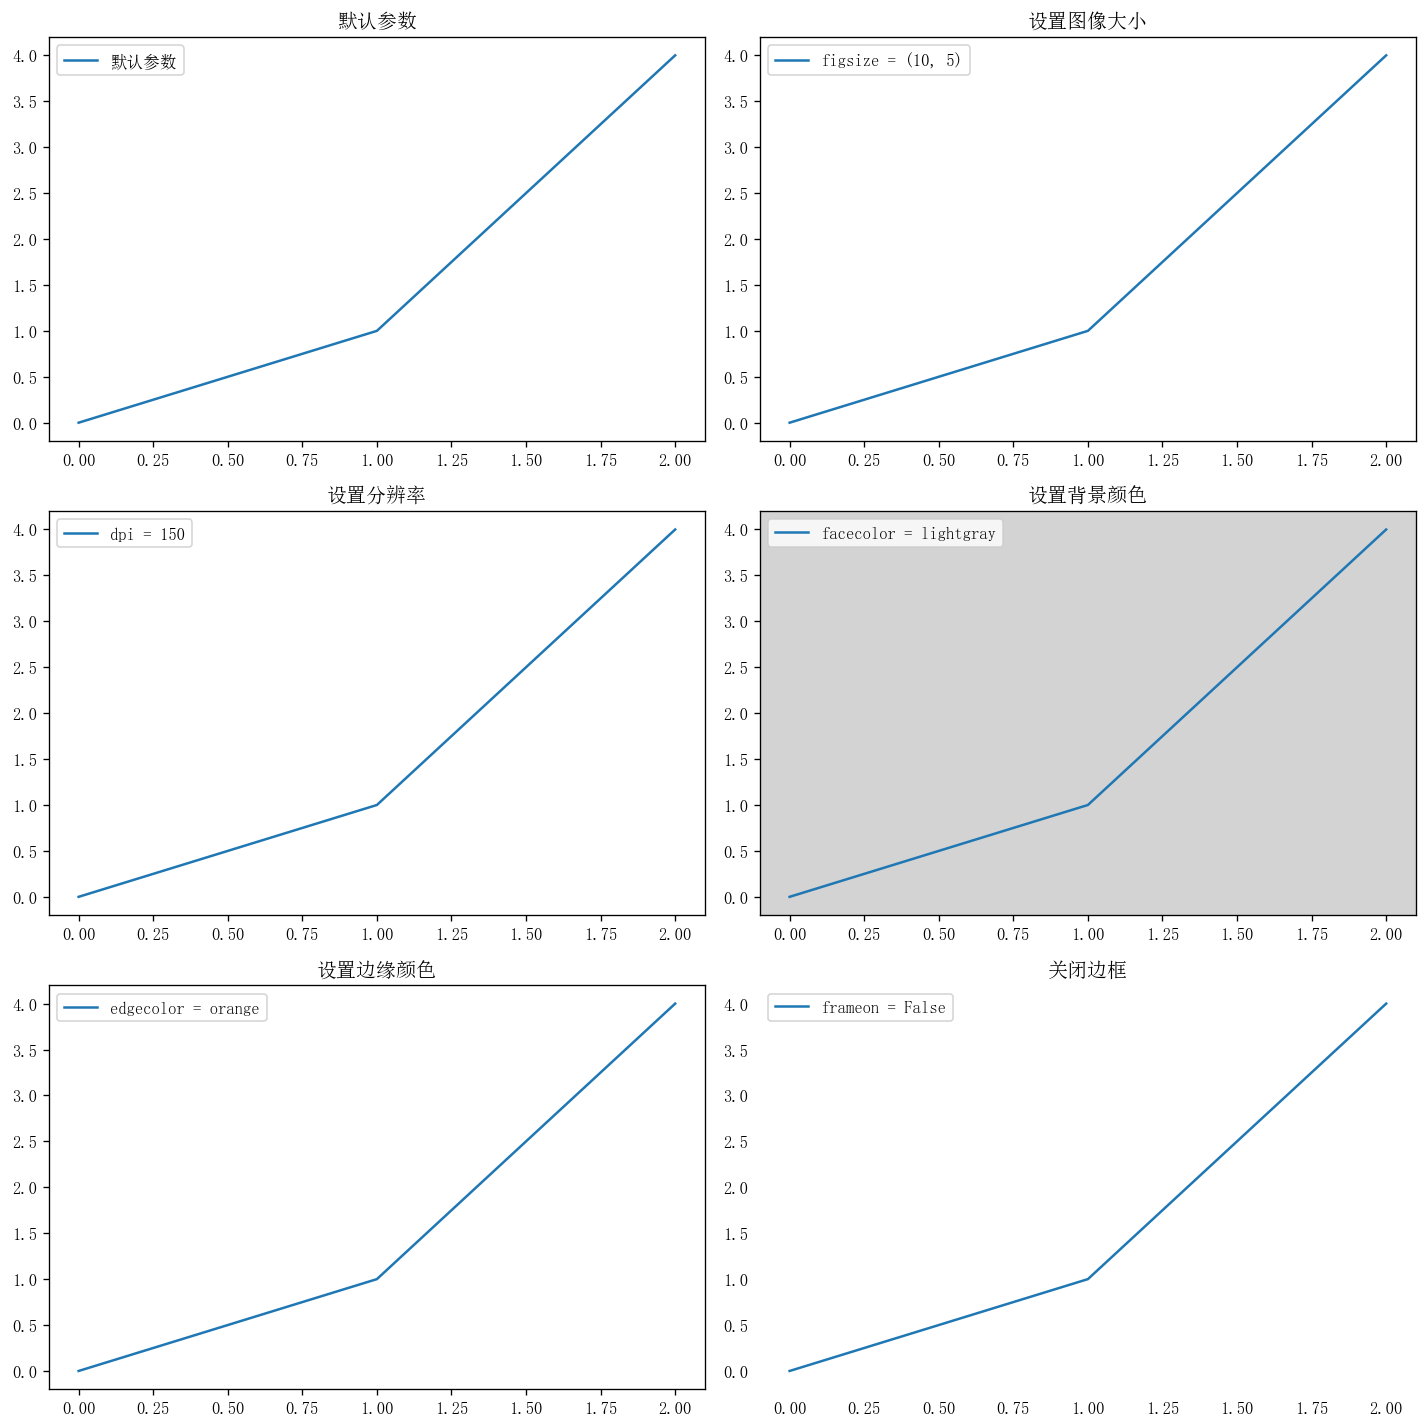
\includegraphics[width=0.8\textwidth]{part/图形化/Matplotlib/pic/图片样式与排版/修改图片参数.png}
    \caption{修改图片参数}
    \label{fig:修改图片参数}
\end{figure}

\section{matplotlib线条}
\subsection{线条的颜色}
matplotlib 支持使用以下缩写字符设置线条的颜色：

\begin{table}[h]
\centering
\caption{线条颜色}
\begin{tabular}{|c|c|}
\hline
\textbf{缩写字符} & \textbf{颜色} \\ \hline
\codeinline{'b'} & blue \\ \hline
\codeinline{'g'} & green \\ \hline
\codeinline{'r'} & red \\ \hline
\codeinline{'c'} & cyan \\ \hline
\codeinline{'m'} & magenta \\ \hline
\codeinline{'y'} & yellow \\ \hline
\codeinline{'k'} & black \\ \hline
\codeinline{'w'} & white \\ \hline
\end{tabular}
\end{table}

\begin{lstlisting}[style=pythonstyle]
import matplotlib.pyplot as plt

# 颜色列表
colors = ['b', 'g', 'r', 'c', 'm', 'y', 'k', 'w']
labels = ['blue', 'green', 'red', 'cyan', 'magenta', 'yellow', 'black', 'white']

plt.figure(figsize=(10, 6))
for i, color in enumerate(colors):
    plt.plot([0, 1, 2], [i, i + 1, i + 2], color=color, label=labels[i])

plt.title('线条的颜色')
plt.legend(loc='upper left')
plt.show()
\end{lstlisting}

\begin{figure}[htpb]
    \centering
    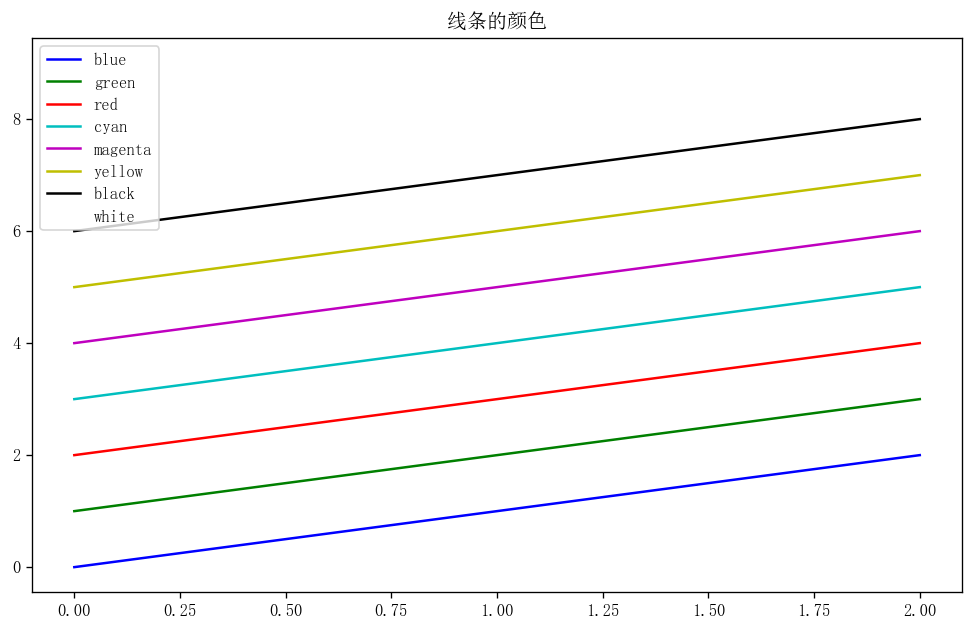
\includegraphics[width=0.6\textwidth]{part/图形化/Matplotlib/pic/图片样式与排版/线条-颜色.png}
    \caption{线条的颜色}
    \label{fig:线条的颜色}
\end{figure}


\subsection{线条的粗细}
线条的粗细可以通过 \codeinline{linewidth} 或 \codeinline{lw} 参数指定，取值为浮点数，表示线条的宽度点数。以下是不同 \codeinline{linewidth} 设置的示例：

\begin{lstlisting}[style=pythonstyle]
import matplotlib.pyplot as plt

# 线条粗细列表
linewidths = [0.5, 1.0, 1.5, 2.0, 2.5, 3.0]

plt.figure(figsize=(10, 6))
for i, lw in enumerate(linewidths):
    # 这里不指定颜色就是使用默认的颜色序列来绘制线条。
    plt.plot([0, 1, 2], [i, i + 1, i + 2], linewidth=lw, label=f'linewidth = {lw}')

plt.title('线条的粗细')
plt.legend(loc='upper left')
plt.show()
\end{lstlisting}

\begin{figure}[htpb]
    \centering
    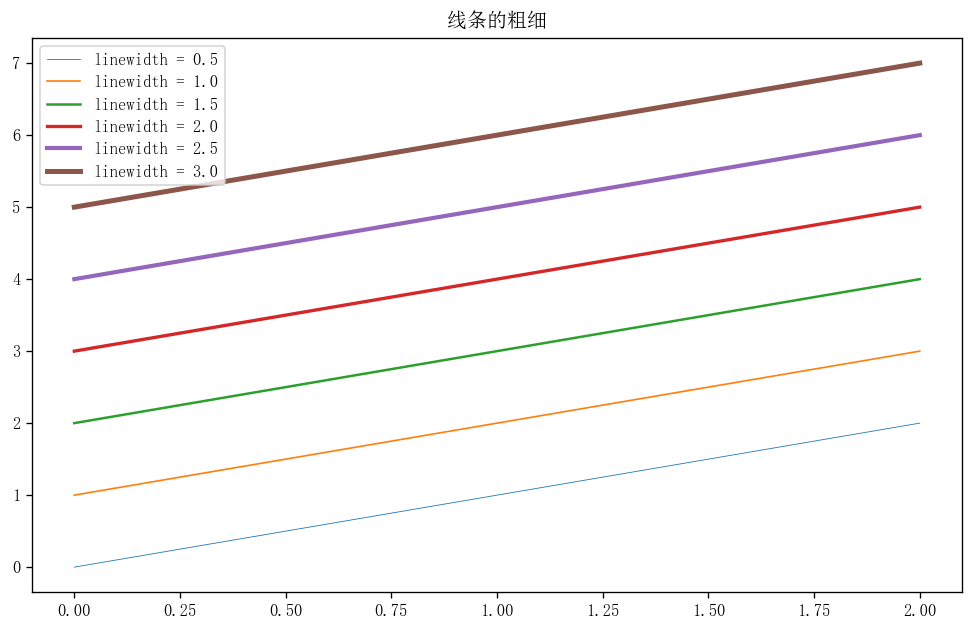
\includegraphics[width=0.6\textwidth]{part/图形化/Matplotlib/pic/图片样式与排版/线条-粗细.png}
    \caption{线条的粗细}
    \label{fig:线条的粗细}
\end{figure}


\subsection{线条的样式}
线条样式可以使用 \codeinline{linestyle} 或 \codeinline{ls} 参数来指定。支持的样式有以下几种：

\begin{table}[h]
\centering
\caption{线条样式}
\begin{tabular}{|c|l|}
\hline
\textbf{样式缩写} & \textbf{描述} \\ \hline
\codeinline{'-'}  & 实线 \\ \hline
\codeinline{'--'} & 短划线 \\ \hline
\codeinline{':' } & 点划线 \\ \hline
\codeinline{'-.'} & 虚线 \\ \hline
\end{tabular}
\end{table}

\begin{lstlisting}[style=pythonstyle]
import matplotlib.pyplot as plt

# 线条样式列表
linestyles = ['-', '--', ':', '-.']
labels = ['实线', '短划线', '点划线', '虚线']

plt.figure(figsize=(10, 6))
for i, ls in enumerate(linestyles):
    plt.plot([0, 1, 2], [i, i + 1, i + 2], linestyle=ls, label=labels[i])

plt.title('线条的样式')
plt.legend(loc='upper left')
plt.show()  
\end{lstlisting}

\begin{figure}[htpb]
    \centering
    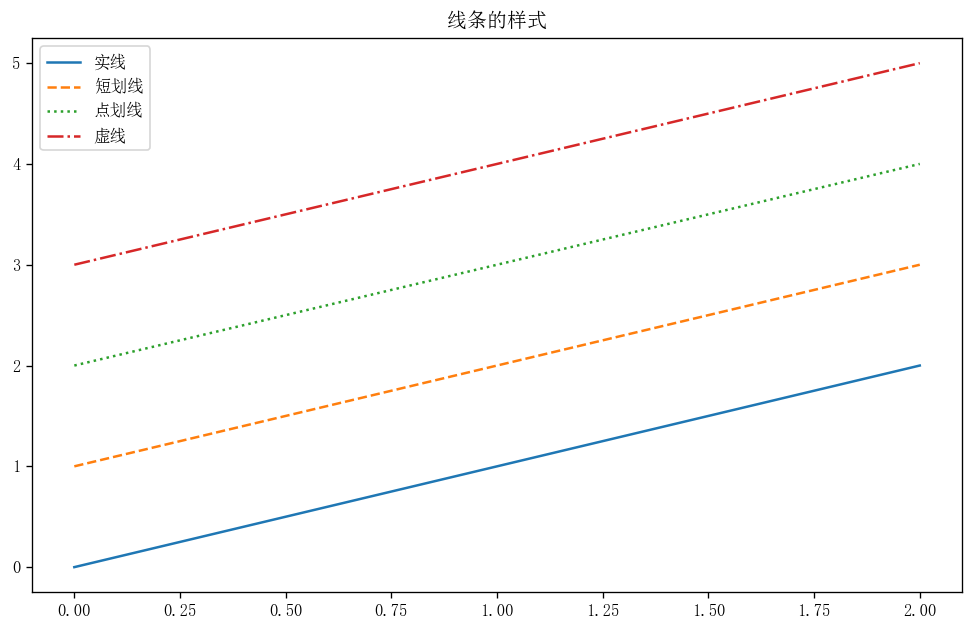
\includegraphics[width=0.6\textwidth]{part/图形化/Matplotlib/pic/图片样式与排版/线条-样式.png}
    \caption{线条的样式}
    \label{fig:线条的样式}
\end{figure}


\subsection{线条的标记}
线条标记是用来在图上标注数据点的符号，可以使用 \codeinline{marker} 参数指定。以下是常用的标记样式：

\begin{table}[h]
\centering
\caption{线条标记}
\begin{tabular}{|c|l|}
\hline
\textbf{标记缩写} & \textbf{描述} \\ \hline
\codeinline{'.'} & 点 (point marker) \\ \hline
\codeinline{','} & 像素 (pixel marker) \\ \hline
\codeinline{'o'} & 圆圈 (circle marker) \\ \hline
\codeinline{'v'} & 向下三角形 (triangle\_down marker) \\ \hline
\codeinline{\textasciicircum} & 向上三角形 (triangle\_up marker) \\ \hline
\codeinline{'<'} & 向左三角形 (triangle\_left marker) \\ \hline
\codeinline{'>'} & 向右三角形 (triangle\_right marker) \\ \hline
\codeinline{'1'} & 下三角 (tri\_down marker) \\ \hline
\codeinline{'2'} & 上三角 (tri\_up marker) \\ \hline
\codeinline{'3'} & 左三角 (tri\_left marker) \\ \hline
\codeinline{'4'} & 右三角 (tri\_right marker) \\ \hline
\codeinline{'s'} & 正方形 (square marker) \\ \hline
\codeinline{'p'} & 五边形 (pentagon marker) \\ \hline
\codeinline{'*'} & 星形 (star marker) \\ \hline
\codeinline{'h'} & 六边形1 (hexagon1 marker) \\ \hline
\codeinline{'H'} & 六边形2 (hexagon2 marker) \\ \hline
\codeinline{'+'} & 加号 (plus marker) \\ \hline
\codeinline{'x'} & 叉号 (x marker) \\ \hline
\codeinline{'D'} & 菱形 (diamond marker) \\ \hline
\codeinline{'d'} & 细菱形 (thin\_diamond marker) \\ \hline
\codeinline{'|'} & 竖线 (vline marker) \\ \hline
\codeinline{'$\_$'} & 横线 (hline marker) \\ \hline
\end{tabular}
\end{table}

\begin{lstlisting}[style=pythonstyle]
import matplotlib.pyplot as plt

# 标记样式列表
markers = ['.', ',', 'o', 'v', '^', '<', '>', '1', '2', '3', '4', 's', 'p', '*', 'h', 'H', '+', 'x', 'D', 'd', '|', '_']
labels = [
    'point', 'pixel', 'circle', 'triangle_down', 'triangle_up', 'triangle_left', 'triangle_right', 
    'tri_down', 'tri_up', 'tri_left', 'tri_right', 'square', 'pentagon', 'star', 'hexagon1', 
    'hexagon2', 'plus', 'x', 'diamond', 'thin_diamond', 'vline', 'hline'
]

plt.figure(figsize=(12, 8))
for i, marker in enumerate(markers):
    plt.plot([0, 1, 2], [i, i + 1, i + 2], marker=marker, label=labels[i])

plt.title('线条的标记')
plt.legend(loc='upper left', fontsize='small')
plt.show()
\end{lstlisting}

\begin{figure}[htpb]
    \centering
    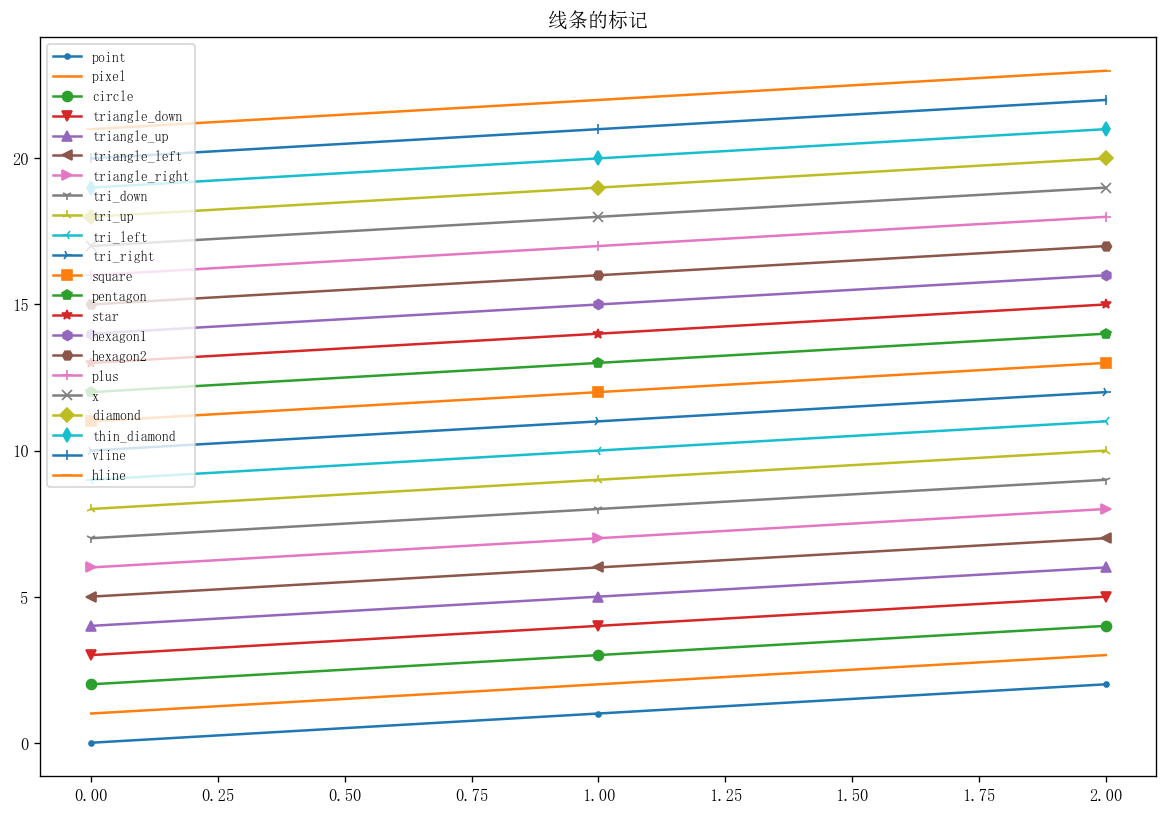
\includegraphics[width=0.6\textwidth]{part/图形化/Matplotlib/pic/图片样式与排版/线条-标记.png}
    \caption{线条的标记}
    \label{fig:线条的标记}
\end{figure}

\begin{lstlisting}[style=pythonstyle]
import matplotlib.pyplot as plt

# 定义标记样式和方向属性
markers = ['o', 'v', '^', '<', '>', '8', 's', 'p', '*', 'h', 'H', 'D', 'd', 'P', 'X']
fillstyles = ['full', 'left', 'right', 'bottom', 'top', 'none']  # 标记的填充样式

# 设置图像大小和子图网格
fig, axs = plt.subplots(len(markers), len(fillstyles), figsize=(12, 18))

# 循环绘制每种标记和填充样式
for i, marker in enumerate(markers):
    for j, fillstyle in enumerate(fillstyles):
        axs[i, j].plot(0, 0, marker=marker, markersize=20, markerfacecolor='orange', fillstyle=fillstyle)
        axs[i, j].set_xticks([])
        axs[i, j].set_yticks([])
        axs[i, j].set_xlim(-1, 1)
        axs[i, j].set_ylim(-1, 1)
        axs[i, j].text(0, 0, f"('{marker}',{fillstyle})", ha='center', va='center')

plt.tight_layout()
plt.show()
\end{lstlisting}


\section{图片的边界}
图片的边界可以通过 \codeinline{plt.xlim()} 和 \codeinline{plt.ylim()} 函数来设置。以下示例展示了如何设置图片的边界：

\begin{lstlisting}[style=pythonstyle]
import matplotlib.pyplot as plt
import numpy as np

# 创建数据
x = np.linspace(-np.pi, np.pi, 100)
y1 = np.sin(x)
y2 = np.cos(x)

# 创建两个子图用于比较
fig, (ax1, ax2) = plt.subplots(1, 2, figsize=(12, 6))

# 第一个子图：默认上下限
ax1.plot(x, y1, color='blue', label='sin(x)')
ax1.plot(x, y2, color='orange', label='cos(x)')
ax1.set_xlim(-np.pi, np.pi)  # 设置 x 轴的上下限
ax1.set_ylim(-1.0, 1.0)      # 设置 y 轴的上下限
ax1.set_title('原始图像')
ax1.legend()

# 第二个子图：扩展 y 轴的上下限 10%
ax2.plot(x, y1, color='blue', label='sin(x)')
ax2.plot(x, y2, color='orange', label='cos(x)')
ax2.set_xlim(-np.pi, np.pi)  # 设置 x 轴的上下限
ax2.set_ylim(-1.1, 1.1)      # 扩展 y 轴的上下限 10%
ax2.set_title('扩展 y 轴上下 10%')
ax2.legend()

# 调整布局并显示图像
plt.tight_layout()
plt.show()
\end{lstlisting}

\begin{figure}[htpb]
    \centering
    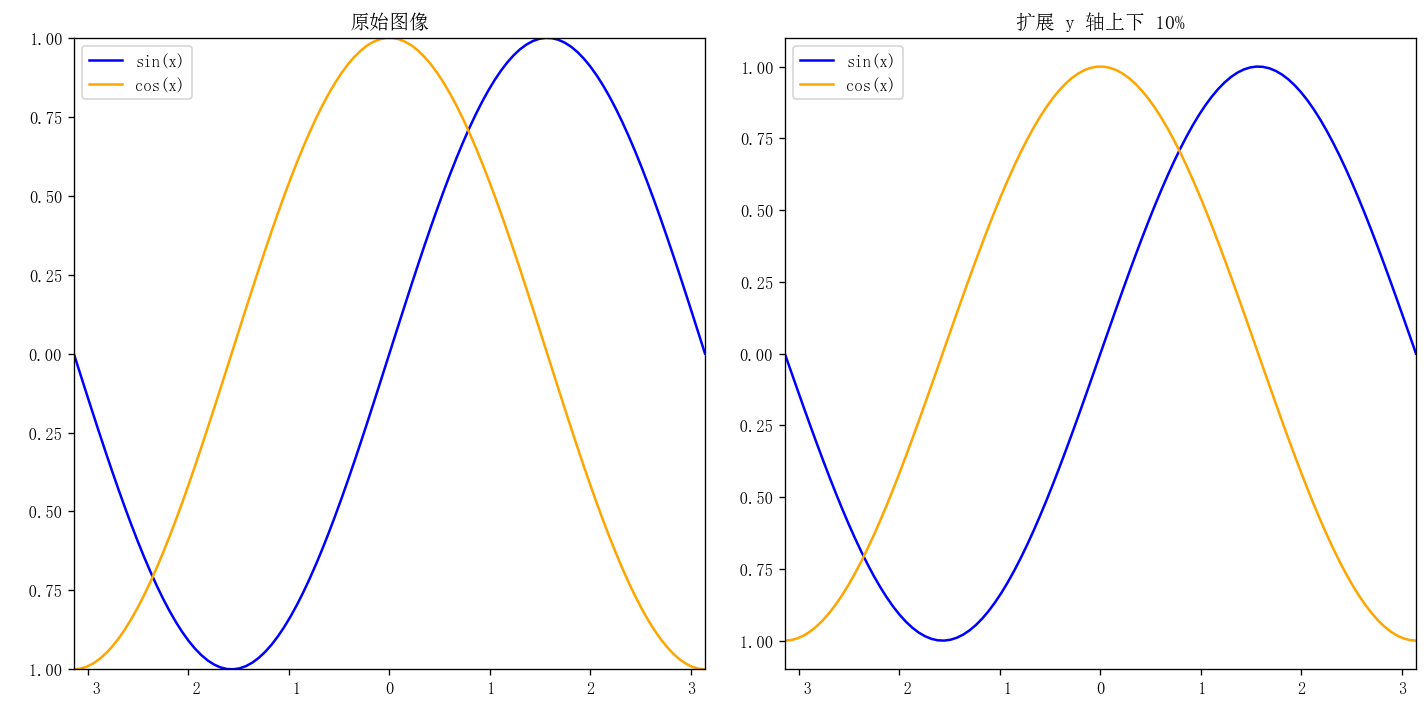
\includegraphics[width=0.6\textwidth]{part/图形化/Matplotlib/pic/图片样式与排版/图片的边界.png}
    \caption{图片的边界}
    \label{fig:图片的边界}
\end{figure}

\section{坐标轴}
\subsection{坐标记号标签}
坐标记号标签通过 \codeinline{plt.xticks()} 和 \codeinline{plt.yticks()} 函数来设置。
其主要功能包括：
\begin{enumerate}[label=\arabic*)]
    \item 设置刻度位置：指定 x 轴上显示刻度的位置。
    \item 设置刻度标签：自定义刻度位置的显示标签，可以使用字符串、数学符号等。
    \item 美化图表：通过设置刻度和标签，可以让图表看起来更加专业、易于理解。
\end{enumerate}

\begin{lstlisting}[style=pythonstyle]
import matplotlib.pyplot as plt
import numpy as np

# 数据
x = np.linspace(-np.pi, np.pi, 100)
y = np.sin(x)

plt.plot(x, y)

# 设置 x 轴的刻度和标签
plt.xticks([-np.pi, -np.pi/2, 0, np.pi/2, np.pi], ['-π', '-π/2', '0', 'π/2', 'π'])
## 第1个参数是刻度的位置，第2个参数是刻度的标签

# 设置 y 轴的刻度和标签
plt.yticks([-1, -0.5, 0, 0.5, 1], ['-1', '-0.5', '0', '0.5', '1'])

plt.title('使用 xticks 和 yticks 设置刻度')
plt.show()
\end{lstlisting}


\begin{lstlisting}[style=pythonstyle]
import matplotlib.pyplot as plt
import numpy as np

# 创建数据
x = np.linspace(-np.pi, np.pi, 100)
y1 = np.sin(x)
y2 = np.cos(x)

# 创建两个子图用于比较
fig, (ax1, ax2) = plt.subplots(1, 2, figsize=(12, 6))

# 第一个子图：不使用 xticks 和 yticks
ax1.plot(x, y1, color='blue', label='sin(x)')
ax1.plot(x, y2, color='orange', label='cos(x)')
ax1.set_title('未设置 xticks 和 yticks')
ax1.legend()

# 第二个子图：使用 xticks 和 yticks
ax2.plot(x, y1, color='blue', label='sin(x)')
ax2.plot(x, y2, color='orange', label='cos(x)')
ax2.set_xticks([-np.pi, -np.pi/2, 0, np.pi/2, np.pi])  # 设置 x 轴刻度
ax2.set_xticklabels(['-π', '-π/2', '0', 'π/2', 'π'])  # 设置 x 轴刻度标签
ax2.set_yticks([-1, -0.5, 0, 0.5, 1])  # 设置 y 轴刻度
ax2.set_yticklabels(['-1', '-0.5', '0', '0.5', '1'])  # 设置 y 轴刻度标签
ax2.set_title('设置 xticks 和 yticks')
ax2.legend()

# 调整布局并显示图像
plt.tight_layout()
plt.show()
\end{lstlisting}
\begin{figure}[htpb]
    \centering
    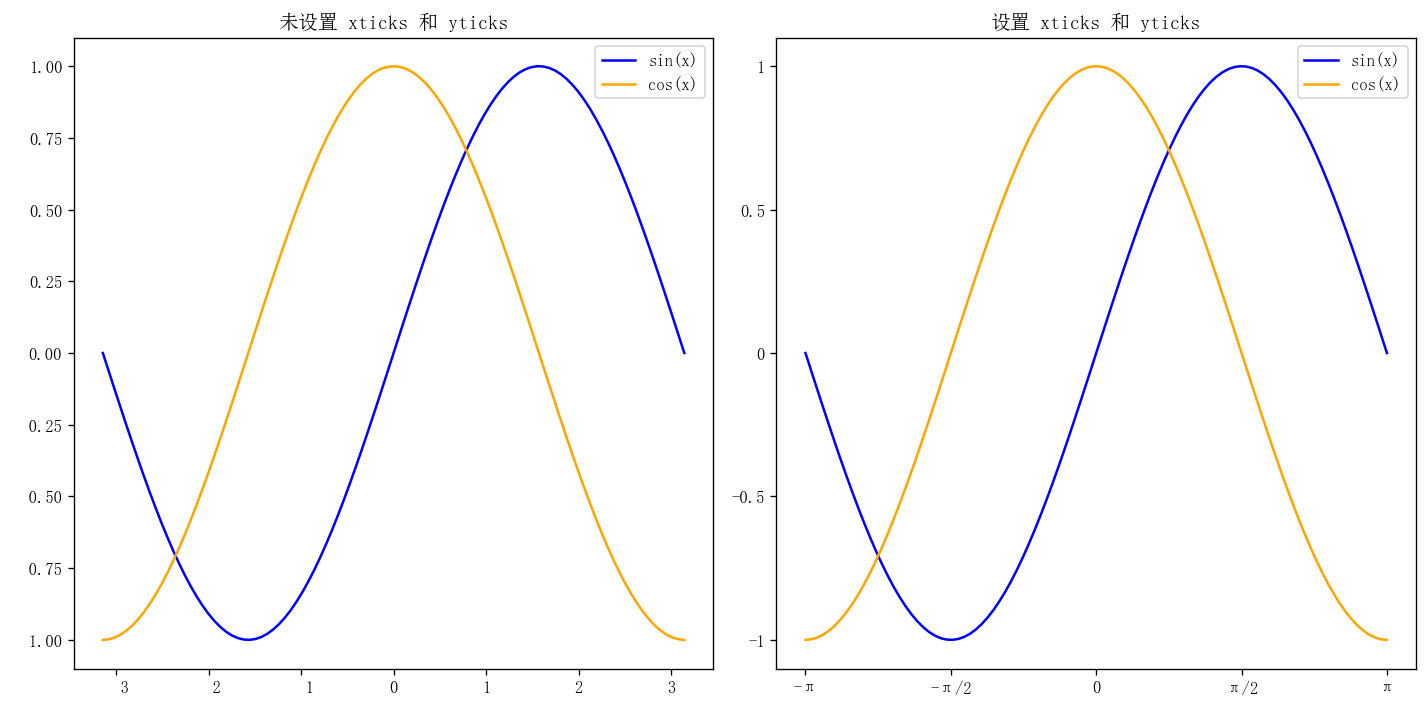
\includegraphics[width=0.6\textwidth]{part/图形化/Matplotlib/pic/图片样式与排版/ticks设置坐标.png}
    \caption{ticks设置坐标}
    \label{fig:ticks设置坐标}
\end{figure}


\subsection{坐标轴的标签}
坐标轴的标签可以通过 \codeinline{plt.xlabel()} 和 \codeinline{plt.ylabel()} 函数来设置。以下示例展示了如何设置坐标轴的标签：

\begin{lstlisting}[style=pythonstyle]
import matplotlib.pyplot as plt
import numpy as np

# 创建数据
x = np.linspace(-np.pi, np.pi, 100)
y1 = np.sin(x)
y2 = np.cos(x)

# 创建两个子图用于比较
fig, (ax1, ax2) = plt.subplots(1, 2, figsize=(12, 6))

# 第一个子图：不使用 xlabel 和 ylabel
ax1.plot(x, y1, color='blue', label='sin(x)')
ax1.plot(x, y2, color='orange', label='cos(x)')
ax1.set_xlim(-np.pi, np.pi)  # 设置 x 轴的上下限
ax1.set_ylim(-1.0, 1.0)      # 设置 y 轴的上下限
ax1.set_title('未设置 xlabel 和 ylabel')
ax1.legend()

# 第二个子图：使用 xlabel 和 ylabel
ax2.plot(x, y1, color='blue', label='sin(x)')
ax2.plot(x, y2, color='orange', label='cos(x)')
ax2.set_xlim(-np.pi, np.pi)  # 设置 x 轴的上下限
ax2.set_ylim(-1.0, 1.0)      # 设置 y 轴的上下限
ax2.set_xlabel('X 轴 (radians)')  # 设置 x 轴标签
ax2.set_ylabel('Y 轴 (value)')    # 设置 y 轴标签
ax2.set_title('设置 xlabel 和 ylabel')
ax2.legend()

# 调整布局并显示图像
plt.tight_layout()
plt.show()
\end{lstlisting}

\begin{figure}[htpb]
    \centering
    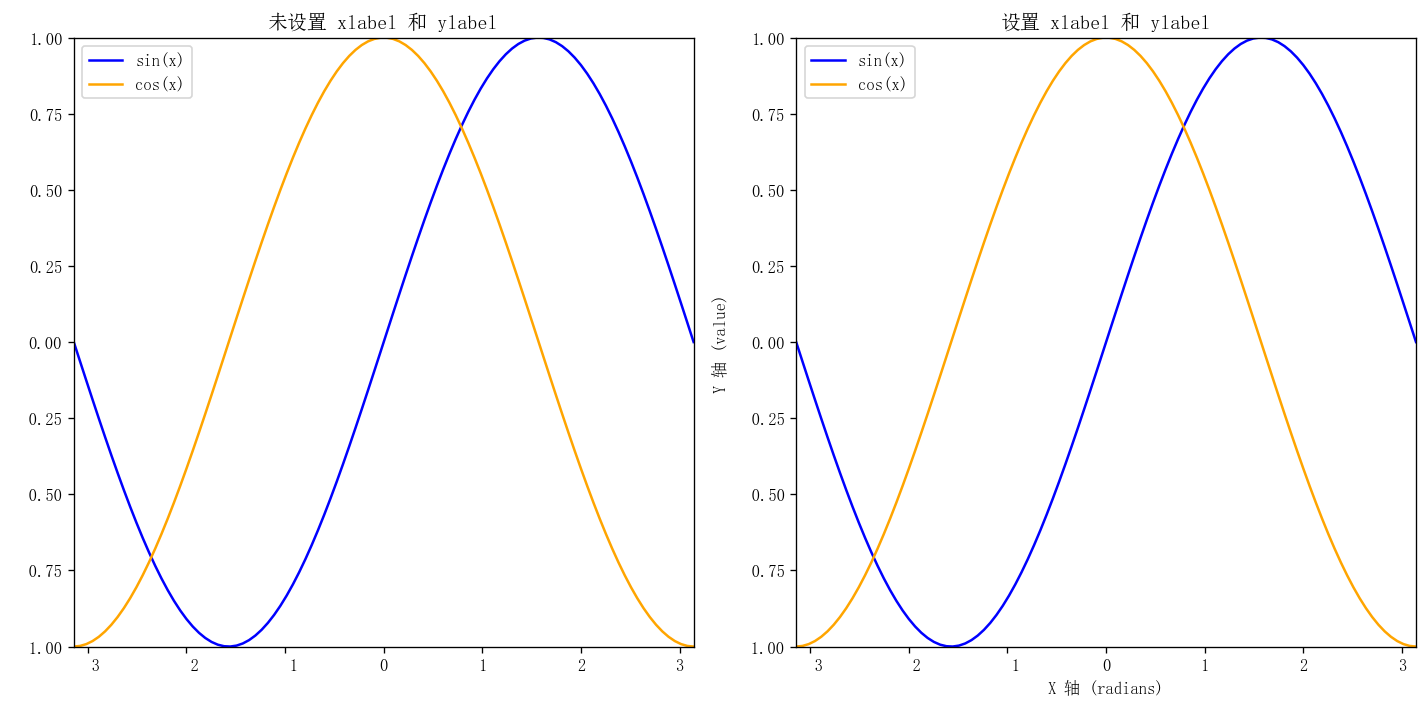
\includegraphics[width=0.6\textwidth]{part/图形化/Matplotlib/pic/图片样式与排版/label标签的设置.png}
    \caption{label标签的设置}
    \label{fig:label标签的设置}
\end{figure}

\subsection{坐标轴移动}
坐标轴线和上面的记号连在一起就形成了脊柱（Spines，一条线段上有一系列的凸起，很像脊柱骨），它记录了数据区域的范围。

默认是放到图的四边，
matplotlib 中的坐标轴线和记号线可以通过 \codeinline{spines} 属性进行设置。以下示例展示了如何将坐标轴移到图的中间：


\begin{lstlisting}[style=pythonstyle]
import matplotlib.pyplot as plt
import numpy as np

# 创建数据
x = np.linspace(-np.pi, np.pi, 100)
y1 = np.sin(x)
y2 = np.cos(x)

# 创建两个子图用于比较
fig, (ax1, ax2) = plt.subplots(1, 2, figsize=(12, 6))

# 第一个子图：默认坐标轴在图的四边
ax1.plot(x, y1, color='blue', label='sin(x)')
ax1.plot(x, y2, color='orange', label='cos(x)')
ax1.set_title('默认坐标轴位置')
ax1.legend()

# 第二个子图：将坐标轴移到图的中间
ax2.plot(x, y1, color='blue', label='sin(x)')
ax2.plot(x, y2, color='orange', label='cos(x)')
ax2.spines['top'].set_color('none')  # 隐藏上边框
ax2.spines['right'].set_color('none')  # 隐藏右边框
ax2.spines['left'].set_position(('data', 0))  # 将左侧的 y 轴移到 x = 0 位置
ax2.spines['bottom'].set_position(('data', 0))  # 将底部的 x 轴移到 y = 0 位置
ax2.set_title('坐标轴移到图的中间')
ax2.legend()

# 调整布局并显示图像
plt.tight_layout()
plt.show()
\end{lstlisting}

\begin{figure}[htpb]
    \centering
    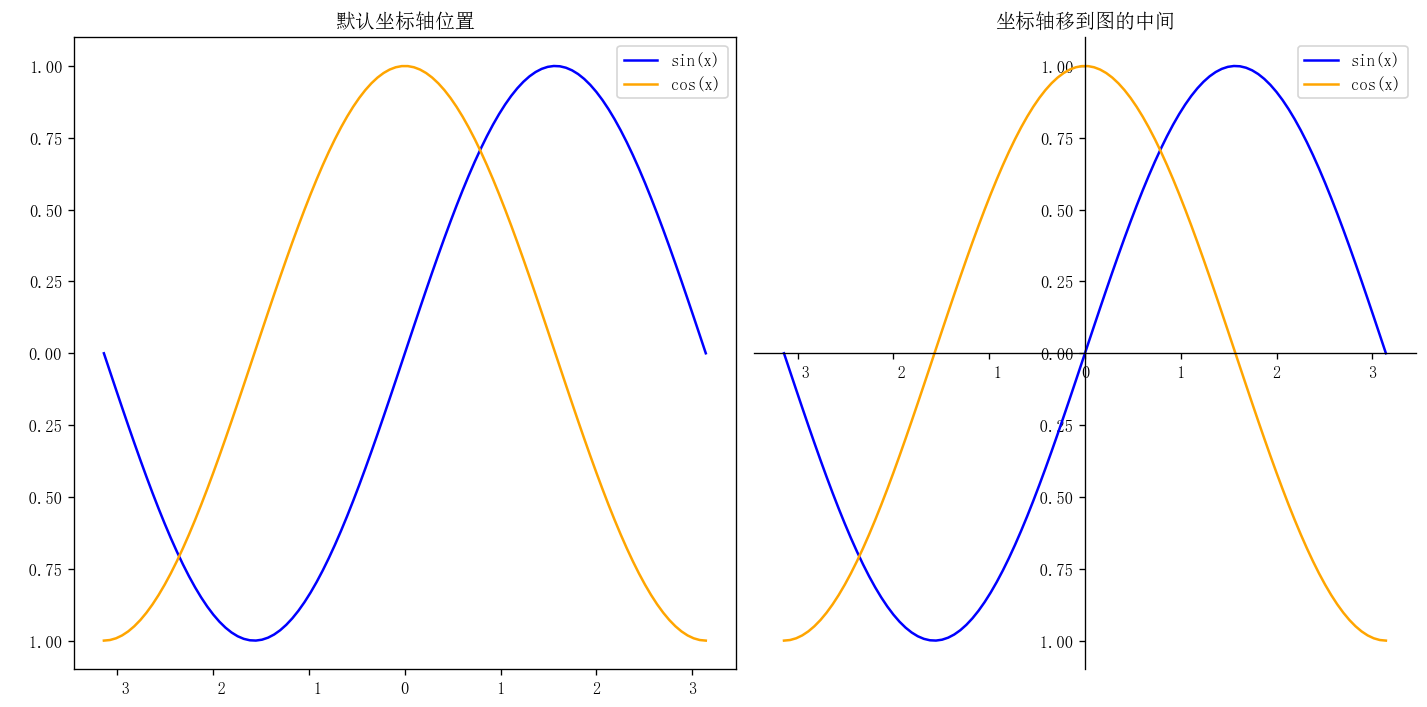
\includegraphics[width=0.6\textwidth]{part/图形化/Matplotlib/pic/图片样式与排版/spines移动坐标轴.png}
    \caption{spines移动坐标轴}
\end{figure}

\subsection{添加图例}
图例是用来区分不同数据的标签，可以通过 \codeinline{plt.legend()} 函数来添加。以下示例展示了如何添加图例：

\begin{lstlisting}[style=pythonstyle]
import matplotlib.pyplot as plt
import numpy as np

# 创建数据
x = np.linspace(-np.pi, np.pi, 100)
y1 = np.sin(x)
y2 = np.cos(x)

# 创建两个子图用于比较
fig, (ax1, ax2) = plt.subplots(1, 2, figsize=(12, 6))

# 第一个子图：不使用图例
ax1.plot(x, y1, color='orange', linewidth=1.0, linestyle='-', label='sin(x)')
ax1.plot(x, y2, color='blue', linewidth=1.0, linestyle='-', label='cos(x)')
ax1.set_title('未添加图例')
# 没有使用 ax1.legend()，因此没有图例

# 第二个子图：使用图例
ax2.plot(x, y1, color='orange', linewidth=1.0, linestyle='-', label='sin(x)')
ax2.plot(x, y2, color='blue', linewidth=1.0, linestyle='-', label='cos(x)')
ax2.set_title('添加图例')
ax2.legend(loc='upper left', fontsize='large')  # 使用图例，放在左上角，字体较大

# 调整布局并显示图像
plt.tight_layout()
plt.show()
\end{lstlisting}
\begin{figure}[htpb]
    \centering
    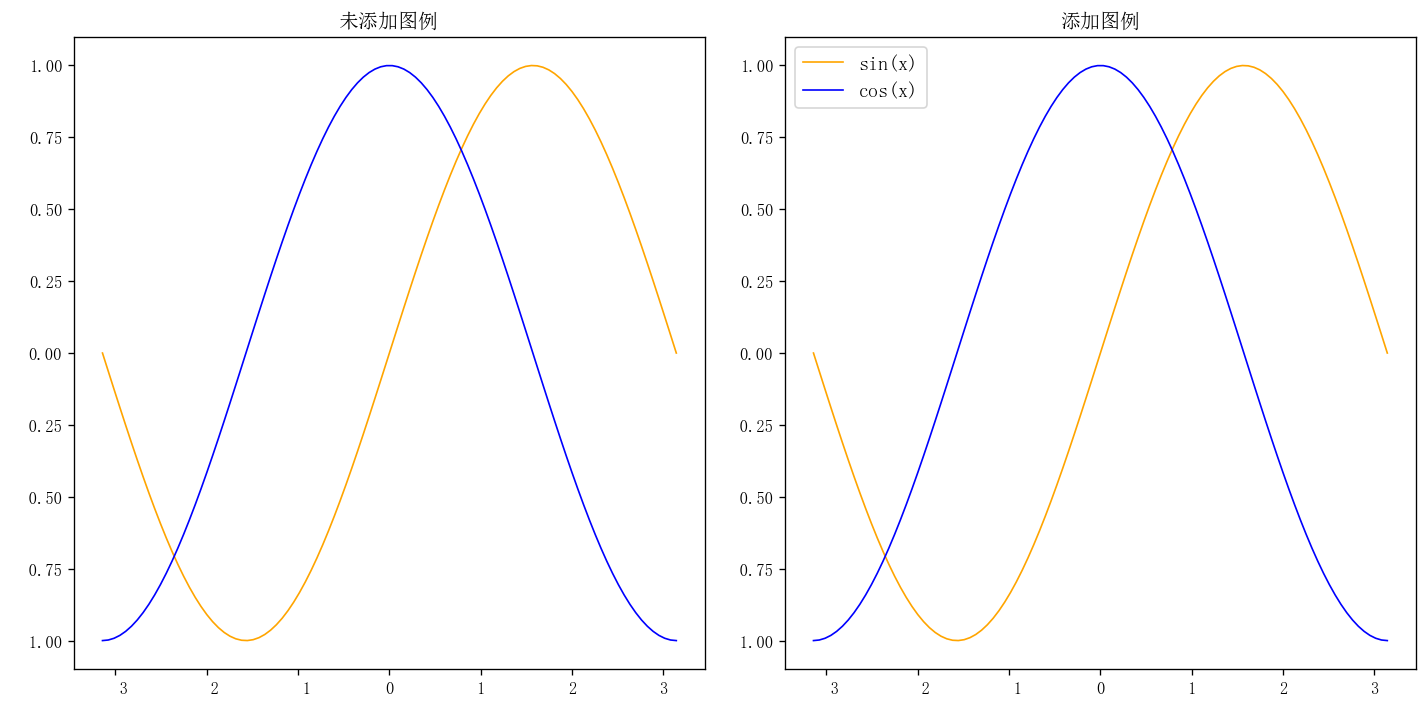
\includegraphics[width=0.6\textwidth]{part/图形化/Matplotlib/pic/图片样式与排版/legend添加图例.png}
    \caption{legend添加图例}
\end{figure}

\subsection{坐标轴的网格}
坐标轴的网格可以通过 \codeinline{plt.grid()} 函数来设置。以下示例展示了如何添加坐标轴的网格：

\begin{lstlisting}[style=pythonstyle]
import matplotlib.pyplot as plt
import numpy as np

# 创建数据
x = np.linspace(-np.pi, np.pi, 100)
y1 = np.sin(x)
y2 = np.cos(x)

# 创建两个子图用于比较
fig, (ax1, ax2) = plt.subplots(1, 2, figsize=(12, 6))

# 第一个子图：不使用网格
ax1.plot(x, y1, color='orange', linewidth=1.0, linestyle='-', label='sin(x)')
ax1.plot(x, y2, color='blue', linewidth=1.0, linestyle='-', label='cos(x)')
ax1.set_title('未使用网格')
ax1.legend(loc='upper left')

# 第二个子图：使用网格
ax2.plot(x, y1, color='orange', linewidth=1.0, linestyle='-', label='sin(x)')
ax2.plot(x, y2, color='blue', linewidth=1.0, linestyle='-', label='cos(x)')
ax2.set_title('使用网格')
ax2.legend(loc='upper left')
ax2.grid(True)  # 开启网格

# 调整布局并显示图像
plt.tight_layout()
plt.show()
\end{lstlisting}
\begin{figure}[htpb]
    \centering
    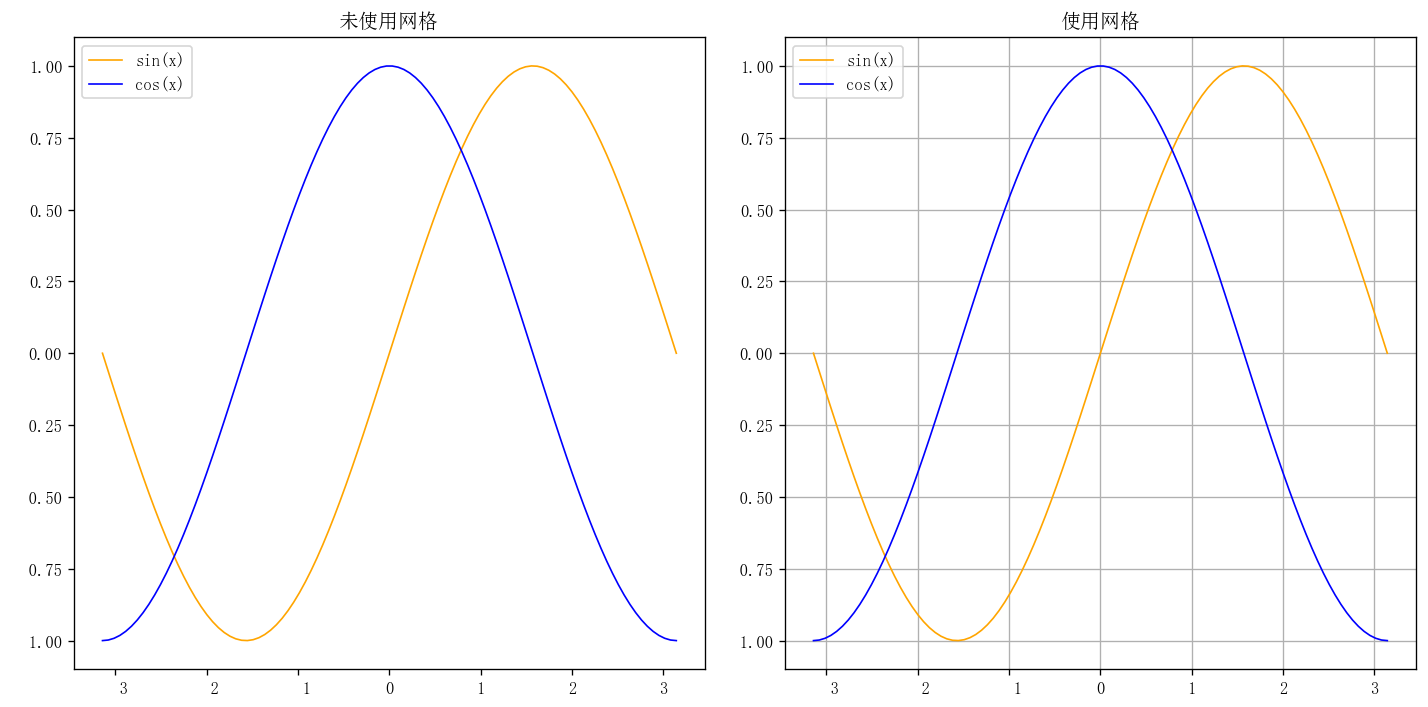
\includegraphics[width=0.6\textwidth]{part/图形化/Matplotlib/pic/图片样式与排版/grid添加网格.png}
    \caption{grid添加网格}
\end{figure}

\subsection{特殊点的注释}
特殊点的注释可以通过 \codeinline{plt.annotate()} 函数来设置。

\codeinline{plt.annotate()} 函数的主要参数包括：
\begin{enumerate}[label=\arabic*)]
    \item \codeinline{s}：注释的内容。
    \item \codeinline{xy}：注释的位置。
    \item \codeinline{xytext}：注释的文本位置。
    \item \codeinline{arrowprops}：箭头的属性。
\end{enumerate}

\begin{lstlisting}[style=pythonstyle]
import matplotlib.pyplot as plt
import numpy as np

# 创建数据
x = np.linspace(-np.pi, np.pi, 100)
y1 = np.sin(x)
y2 = np.cos(x)
t = 2 * np.pi / 3  # 特殊点的位置
t2 = -2 * np.pi / 3  # 特殊点的位置

# 创建两个子图用于比较
fig, (ax1, ax2) = plt.subplots(1, 2, figsize=(14, 6))

# 第一个子图：不添加注释
ax1.plot(x, y1, color='orange', linewidth=1.5, linestyle='-', label='sin(x)')
ax1.plot(x, y2, color='blue', linewidth=1.5, linestyle='-', label='cos(x)')
ax2.scatter([t2], [np.cos(t2)], 30, color='blue') # 添加特殊点
ax1.scatter([t], [np.sin(t)], 30, color='orange') # 添加特殊点
ax1.set_title('未添加注释')
ax1.axhline(0, color='black', linewidth=0.5) 
ax1.axvline(0, color='black', linewidth=0.5) 
ax1.legend(loc='upper left')

# 第二个子图：添加注释
ax2.plot(x, y1, color='orange', linewidth=1.5, linestyle='-', label='sin(x)')
ax2.plot(x, y2, color='blue', linewidth=1.5, linestyle='-', label='cos(x)')
ax2.scatter([t2], [np.cos(t2)], 30, color='blue')
ax2.scatter([t], [np.sin(t)], 30, color='orange')
ax2.set_title('添加注释')
ax2.axhline(0, color='black', linewidth=0.5)
ax2.axvline(0, color='black', linewidth=0.5)

# 添加注释
ax2.annotate(r'$\sin(\frac{2\pi}{3})=\frac{\sqrt{3}}{2}$',
             xy=(t, np.sin(t)), xycoords='data',
             xytext=(+10, +30), textcoords='offset points', fontsize=16,
             arrowprops=dict(arrowstyle="->", connectionstyle="arc3,rad=.2"))

ax2.annotate(r'$\cos(-\frac{2\pi}{3})=-\frac{1}{2}$',
             xy=(t2, np.cos(t2)), xycoords='data',
             xytext=(-90, 0), textcoords='offset points', fontsize=16,
             arrowprops=dict(arrowstyle="->", connectionstyle="arc3,rad=.2"))

ax2.legend(loc='upper left')

# 调整布局并显示图像
plt.tight_layout()
plt.show()
\end{lstlisting}
\begin{figure}[htpb]
    \centering
    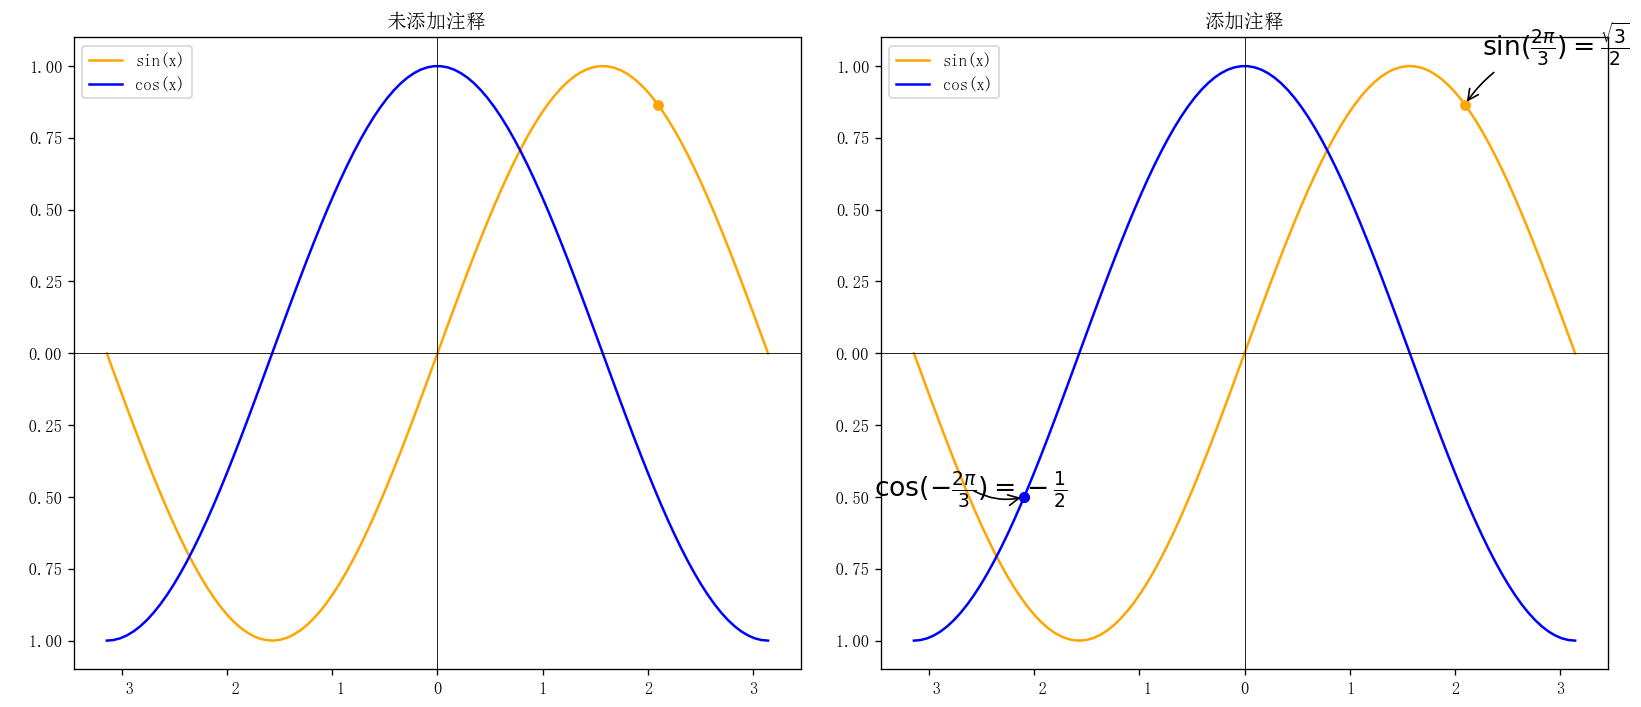
\includegraphics[width=0.6\textwidth]{part/图形化/Matplotlib/pic/图片样式与排版/annotation添加注释.png}
    \caption{annotation添加注释}
\end{figure}



\section{箭头}
箭头可以通过 \codeinline{plt.arrow()} 函数来设置。以下示例展示了如何添加箭头：

\begin{lstlisting}[style=pythonstyle]
import matplotlib.pyplot as plt

# 创建图像
plt.figure(figsize=(8, 6))

# 绘制箭头
plt.arrow(0, 0, 0.5, 0.5, width=0.02, head_width=0.1, head_length=0.1, fc='blue', ec='black')
## 从 (0, 0) 开始，到 (0.5, 0.5) 结束
## width 是箭头的宽度，head_width 是箭头的底部宽度，head_length 是箭头的长度
## fc 是箭头的填充颜色，ec 是箭头的边框颜色

plt.text(0.6, 0.6, '箭头', fontsize=12, color='black', ha='center', va='center')

# 设置坐标轴
plt.xlim(-1, 1)
plt.ylim(-1, 1)

# 添加标题
plt.title('示例：使用 plt.arrow() 添加箭头')

# 显示图像
plt.grid(True)
plt.show()
\end{lstlisting}    


\section{图片风格}
matplotlib 提供了一些预设的风格，
\begin{lstlisting}[style=demostyle, numbers=none]
print(plt.style.available[:])
>>>
['bmh', 'classic', 'dark_background', 'fivethirtyeight', 'ggplot']
\end{lstlisting}

可以通过 \codeinline{plt.style.use()} 函数来设置。以下示例展示了如何设置图片风格：

\begin{lstlisting}[style=pythonstyle]
import matplotlib.pyplot as plt
import numpy as np

# 数据生成
x = np.linspace(0, 10, 100)
y1 = np.sin(x)
y2 = np.cos(x)

# 定义绘图风格
styles = ['Solarize_Light2', '_classic_test_patch', '_mpl-gallery', '_mpl-gallery-nogrid', 
          'bmh', 'classic', 'dark_background', 'fast', 'fivethirtyeight', 'ggplot', 
          'grayscale', 'seaborn-v0_8', 'seaborn-v0_8-bright', 'seaborn-v0_8-colorblind', 
          'seaborn-v0_8-dark', 'seaborn-v0_8-dark-palette', 'seaborn-v0_8-darkgrid', 
          'seaborn-v0_8-deep', 'seaborn-v0_8-muted', 'seaborn-v0_8-notebook', 
          'seaborn-v0_8-paper', 'seaborn-v0_8-pastel', 'seaborn-v0_8-poster', 
          'seaborn-v0_8-talk', 'seaborn-v0_8-ticks', 'seaborn-v0_8-white', 
          'seaborn-v0_8-whitegrid', 'tableau-colorblind10']

# 计算行数和列数，每行3个
n_cols = 3
n_rows = (len(styles) + n_cols - 1) // n_cols  # 计算需要的行数

# 创建图和子图
fig, axs = plt.subplots(n_rows, n_cols, figsize=(10, n_rows * 3))
axs = axs.flatten()  # 展平成一维数组便于遍历

# 绘制每种风格
for i, style in enumerate(styles):
    plt.style.use(style)  # 设置当前风格
    axs[i].plot(x, y1, label='sin(x)')
    axs[i].plot(x, y2, label='cos(x)')
    axs[i].set_title(f'Style: {style}', fontsize=10)
    axs[i].legend(loc='upper right', fontsize=8)
    axs[i].grid(True)

# 隐藏多余的子图
for j in range(len(styles), len(axs)):
    axs[j].axis('off')

# 调整布局
plt.tight_layout()
plt.show()
\end{lstlisting}    
\begin{figure}[htpb]
    \centering
    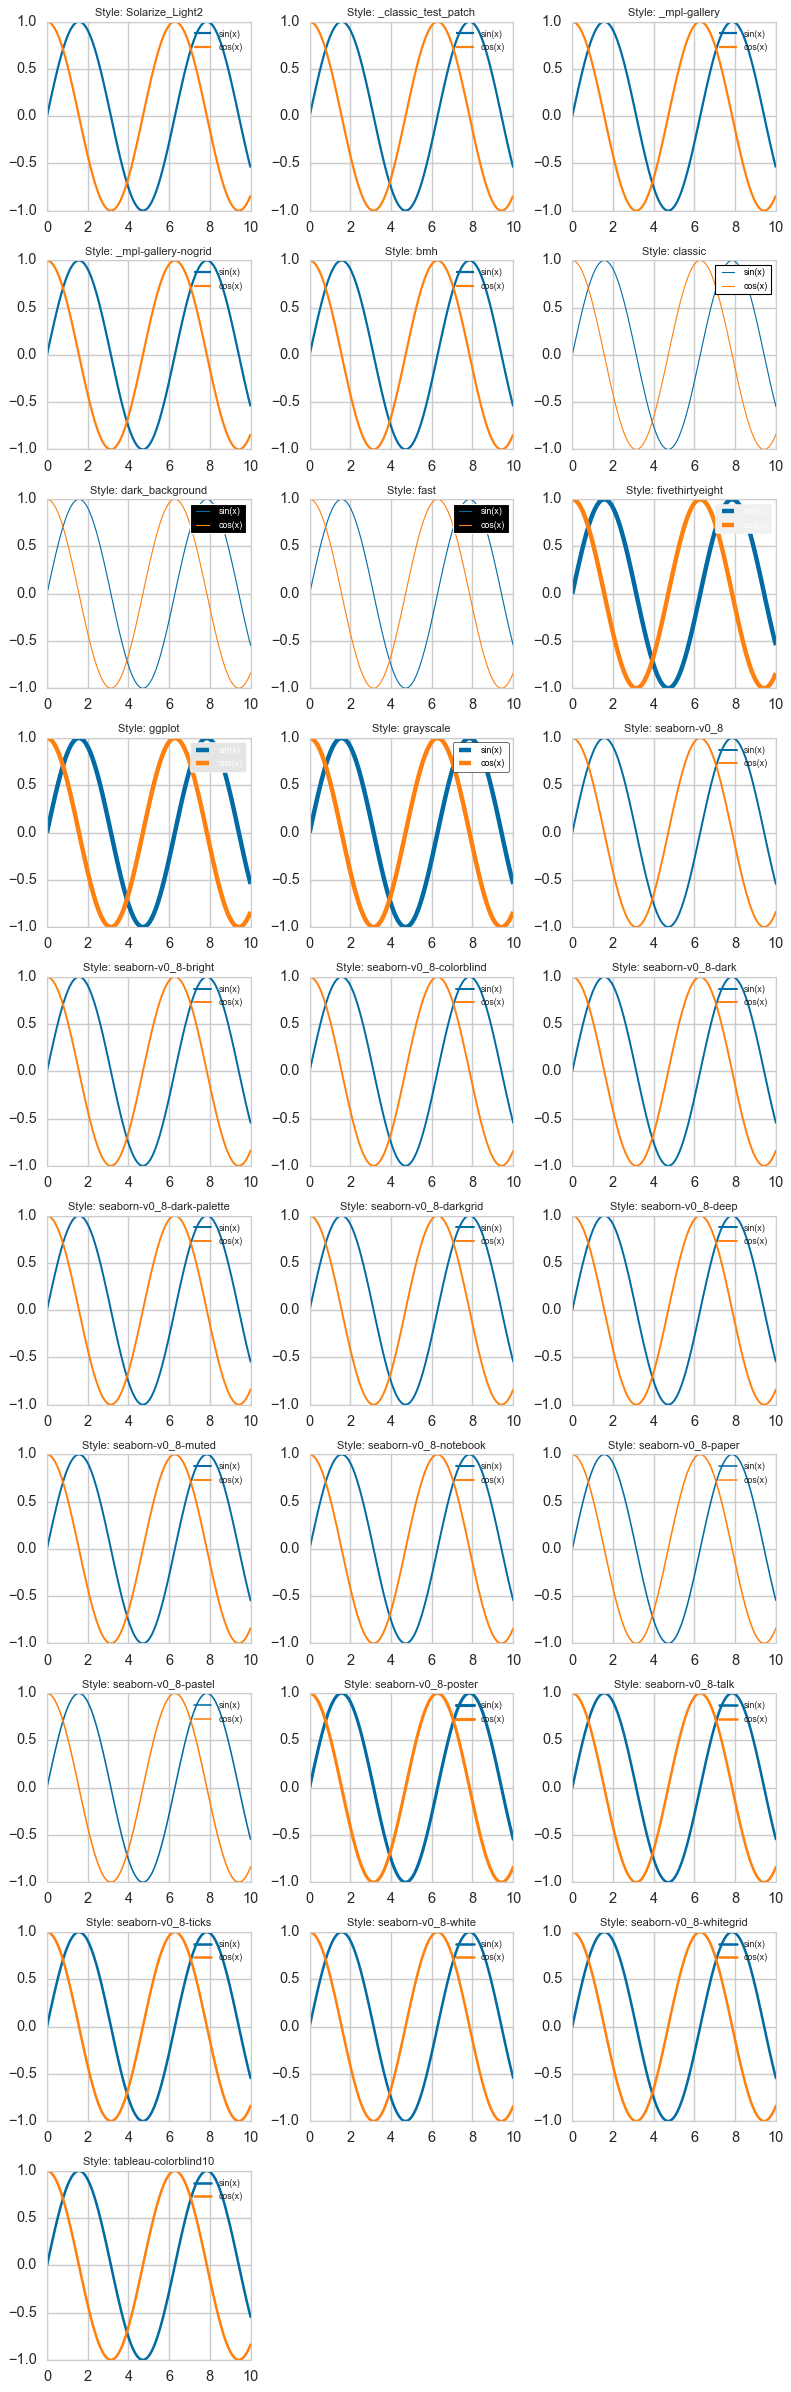
\includegraphics[width=0.6\textwidth]{part/图形化/Matplotlib/pic/图片样式与排版/style设置绘图风格.png}
    \caption{style设置绘图风格}
\end{figure}


\section{多图的排列}
Matplotlib 提供了多种方法来绘制子图，常用的方法包括 
\codeinline{plt.subplot()}、\codeinline{plt.subplots()} 和 \codeinline{GridSpec}。

\subsection{plt.subplot()}
\codeinline{plt.subplot()} 可以快速创建子图。
\begin{lstlisting}[style=demostyle, numbers=none]
plt.subplot(nrows, ncols, index)
# nrows：子图的行数
# ncols：子图的列数
# index：子图的索引，从1开始
\end{lstlisting}

\begin{lstlisting}[style=pythonstyle]
import matplotlib.pyplot as plt
import numpy as np

# 创建数据
x = np.linspace(0, 10, 100)
y1 = np.sin(x)
y2 = np.cos(x)

# 创建一个2行1列的子图布局，绘制第一个子图
plt.subplot(2, 1, 1) # 创建一个2行1列的布局，子图在第1个位置
plt.plot(x, y1)
plt.title('Sine Function')

# 创建一个2行1列的子图布局，绘制第二个子图
plt.subplot(2, 1, 2)
plt.plot(x, y2)
plt.title('Cosine Function')

# 显示图像
plt.tight_layout()  # 自动调整子图间距
plt.show()
\end{lstlisting}
\begin{figure}[htpb]
    \centering
    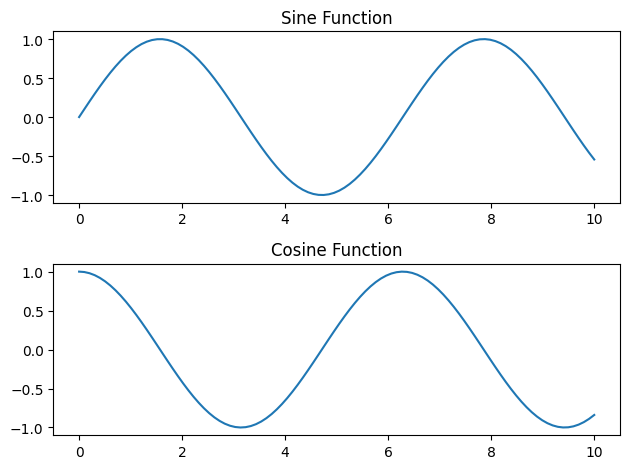
\includegraphics[width=0.4\textwidth]{part/图形化/Matplotlib/pic/图片样式与排版/plt.subplot创建子图演示.png}
    \caption{plt.subplot()创建子图演示}
\end{figure}

\subsubsection{add\_subplot()添加子图}
\codeinline{plt.subplot()} 函数返回的是当前子图对象，可以通过 \codeinline{add\_subplot()} 方法来添加子图。
\begin{lstlisting}[style=demostyle, numbers=none]
ax = fig.add_subplot(nrows, ncols, index)
# nrows：子图的行数
# ncols：子图的列数
# index：子图的索引，从1开始
\end{lstlisting}

\begin{lstlisting}[style=pythonstyle]
import numpy as np
import matplotlib.pyplot as plt

# 创建数据
rad = np.arange(0, np.pi * 2, 0.01)

# 创建图形对象 p1
p1 = plt.figure(figsize=(8, 10), dpi=80)  # 确定画布大小

# 第一个子图
ax1 = p1.add_subplot(2, 1, 1)  # 创建一个两行1列的子图，并开始绘制第一幅
plt.title('lines')  # 添加标题
plt.xlabel('x1')  # 添加x轴的名称
plt.ylabel('y1')  # 添加y轴的名称
plt.xlim((0, 1))  # 确定x轴范围
plt.ylim((0, 1))  # 确定y轴范围
plt.xticks([0, 0.2, 0.4, 0.6, 0.8, 1])  # 规定x轴刻度
plt.yticks([0, 0.2, 0.4, 0.6, 0.8, 1])  # 确定y轴刻度
plt.plot(rad, rad)  # 添加 y = x 曲线
plt.plot(rad, rad**2)  # 添加 y = x^2 曲线
plt.legend(['y=x', 'y=x^2'])

# 第二个子图
ax2 = p1.add_subplot(2, 1, 2)  # 开始绘制第2幅
plt.title('sin/cos')  # 添加标题
plt.xlabel('x2')  # 添加x轴的名称
plt.ylabel('y2')  # 添加y轴的名称
plt.xlim((0, np.pi * 2))  # 确定x轴范围
plt.ylim((-1, 1))  # 确定y轴范围
plt.xticks([0, np.pi / 2, np.pi, np.pi * 1.5, np.pi * 2])  # 规定x轴刻度
plt.yticks([-1, -0.5, 0, 0.5, 1])  # 确定y轴刻度
plt.plot(rad, np.sin(rad))  # 添加 sin 曲线
plt.plot(rad, np.cos(rad))  # 添加 cos 曲线
plt.legend(['sin', 'cos'])

# 保存并显示图像
plt.savefig('../tmp/subplot通过add_subplot添加子图.png')
plt.show()
\end{lstlisting}

\begin{figure}[htpb]
    \centering
    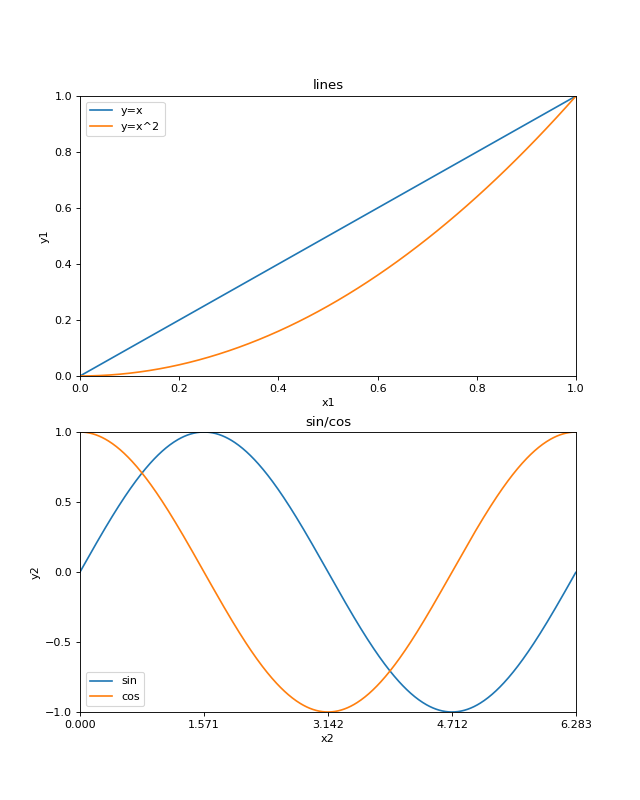
\includegraphics[width=0.4\textwidth]{part/图形化/Matplotlib/pic/图片样式与排版/subplot通过add_subplot添加子图.png}
    \caption{subplot通过add\_subplot添加子图}
\end{figure}




\subsection{plt.subplots()}
\codeinline{plt.subplots()} 是 Matplotlib 中创建子图的推荐方法，它返回一个图形对象和一个包含所有子图的数组对象。
\begin{lstlisting}[style=demostyle, numbers=none]
fig, axs = plt.subplots(nrows, ncols)
# nrows：子图的行数
# ncols：子图的列数
\end{lstlisting}

\begin{lstlisting}[style=pythonstyle]
import matplotlib.pyplot as plt
import numpy as np

# 创建数据
x = np.linspace(0, 10, 100)
y1 = np.sin(x)
y2 = np.cos(x)

# 使用 subplots 创建 1行2列的子图布局
fig, axs = plt.subplots(1, 2, figsize=(10, 4))

# 绘制第一个子图
axs[0].plot(x, y1, 'r-')
axs[0].set_title('Sine Function')

# 绘制第二个子图
axs[1].plot(x, y2, 'b-')
axs[1].set_title('Cosine Function')

# 调整子图布局
plt.tight_layout()
plt.show()
\end{lstlisting}
\begin{figure}[htpb]
    \centering
    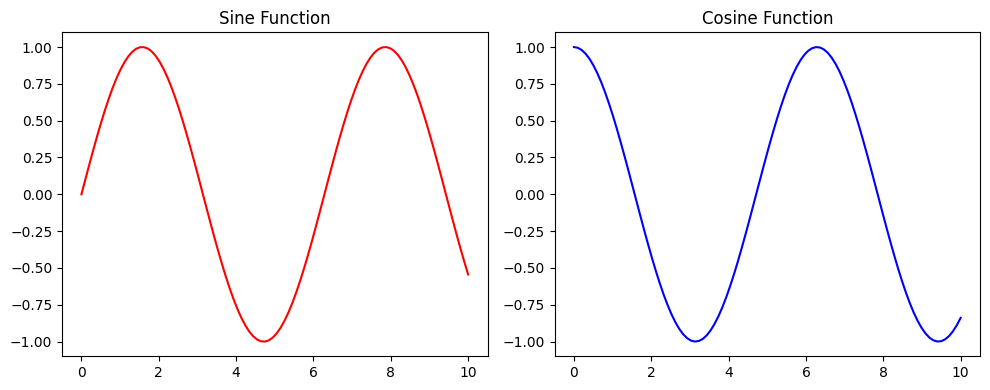
\includegraphics[width=0.4\textwidth]{part/图形化/Matplotlib/pic/图片样式与排版/plt.subplots创建子图演示.png}
    \caption{plt.subplots()创建子图演示}
\end{figure}


\subsection{GridSpec}
\codeinline{GridSpec} 提供了更灵活的方式来创建复杂的子图布局。
通过 \codeinline{GridSpec} 可以更细致地控制子图的大小和位置。
\begin{lstlisting}[style=demostyle, numbers=none]
from matplotlib.gridspec import GridSpec
gs = GridSpec(nrows, ncols)
# nrows：子图的行数
# ncols：子图的列数

ax = fig.add_subplot(gs[row, col])
# gs[row, col]：获取第 row 行第 col 列的子图
# row：子图的行索引，从0开始
# col：子图的列索引，从0开始
\end{lstlisting}

\begin{lstlisting}[style=pythonstyle]
import matplotlib.pyplot as plt
import numpy as np
from matplotlib.gridspec import GridSpec

# 创建数据
x = np.linspace(0, 10, 100)
y1 = np.sin(x)
y2 = np.cos(x)
y3 = np.tan(x)

# 创建一个新的图形
fig = plt.figure(figsize=(8, 6))

# 创建一个2x2的网格布局
gs = GridSpec(2, 2, figure=fig)

# 绘制子图1，占据第1行的全部
ax1 = fig.add_subplot(gs[0, :])
ax1.plot(x, y1, 'g-')
ax1.set_title('Sine Function')

# 绘制子图2，占据第2行第1列
ax2 = fig.add_subplot(gs[1, 0])
ax2.plot(x, y2, 'r-')
ax2.set_title('Cosine Function')

# 绘制子图3，占据第2行第2列
ax3 = fig.add_subplot(gs[1, 1])
ax3.plot(x, y3, 'b-')
ax3.set_title('Tangent Function')

# 调整子图布局
plt.tight_layout()
plt.show()
\end{lstlisting}
\begin{figure}[htpb]
    \centering
    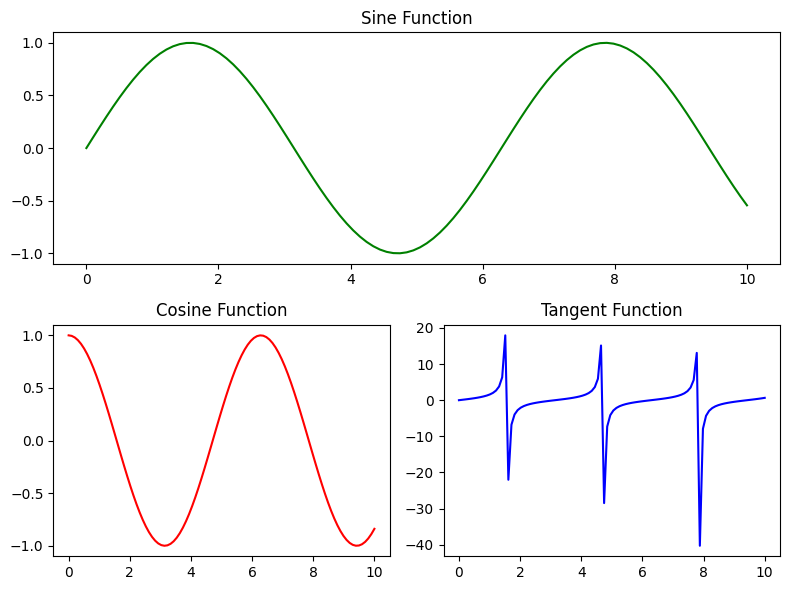
\includegraphics[width=0.4\textwidth]{part/图形化/Matplotlib/pic/图片样式与排版/GridSpec创建子图演示.png}
    \caption{GridSpec创建子图演示}
\end{figure}


\subsection{自定义子图大小和间距}
使用 \codeinline{plt.subplots\_adjust()} 可以调整子图之间的间距，方便对布局进行微调。
\begin{lstlisting}[style=demostyle, numbers=none]
plt.subplots_adjust(left=None, bottom=None, right=None, top=None, wspace=None, hspace=None)
# left：左边距比例，默认为0.125
# bottom：下边距比例，默认为0.11
# right：右边距比例，默认为0.9
# top：上边距比例，默认为0.88
# wspace：水平间距比例，默认为0.2
# hspace：垂直间距比例，默认为0.2
\end{lstlisting}

\begin{lstlisting}[style=pythonstyle]
import matplotlib.pyplot as plt
import numpy as np

# 创建数据
x = np.linspace(0, 10, 100)
y1 = np.sin(x)
y2 = np.cos(x)

# 创建一个2x1的子图
fig, (ax1, ax2) = plt.subplots(2, 1, figsize=(8, 6))

# 绘制子图
ax1.plot(x, y1, 'm-')
ax1.set_title('Sine Function')

ax2.plot(x, y2, 'c-')
ax2.set_title('Cosine Function')

# 调整子图之间的间距
plt.subplots_adjust(hspace=0.4, wspace=0.3)
plt.show()
\end{lstlisting}


